\chapter{DOMAIN ANALYSIS}

There must be at least a single paragraph between a chapter and a section.
Here you can simply summarize the chapter, like "In this chapter we will do this and that".

\section{Problem Definition}

Here you explain why you've decided to do this thesis project.
Was there no existing solution for a problem?
Did you have an idea on how to improve an existing solution?
Or perhaps you simply wanted to check a hypothesis,
like "is JS a good language for building a nuclear reactor"?

Notice how the section titles use Title Case.
We weren't given any strict rules, but basically:
\begin{itemize}
\item capitalize the principal words;
\item capitalize prepositions and conjunctions of four letters or more;
\item lowercase the articles the, a, and an.
\end{itemize}

By the way, here is how to write simple lists:
\begin{itemize}
    \item first later is lowercase;
    \item semicolon at the end;
    \item period at the end of last item.
\end{itemize}

Cite your sources, and if you don't have any sources, do your research first!
Here are some popular scientific papers \cite{Sarkar2020OAuth, mcculloch1943logical,shannon1948mathematical,rumelhart1986learning,vaswani2017attention},
articles \cite{he2016deep,brooks1987no,turing1950computing,dijkstra1968go,cerf1974protocol}
and books \cite{knuth1974structured,knuth1997art,cormen2009introduction,aima2020,sipser2012introduction,tanenbaum2006structured}
to showcase the bibliography formatting.

\section{Some Technical Concept}

The next section can be an introduction to some technical concepts that your topic requires.
Use diagrams, either your own or from the internet (in which case you have to cite them).

Floats (figures, tables and code listings) are not allowed to be at the top of the page,
there should be at least a few lines separating them from the top.
Also, they may not touch each other, there should be at least a few lines separating them.
Look up how to use \verb|[!hb]| after \verb|\begin{figure}|, 
this way Latex will aid you in placing them according to these rules.

\subsection{Subsection Example}

\begin{figure}[h]
\centering
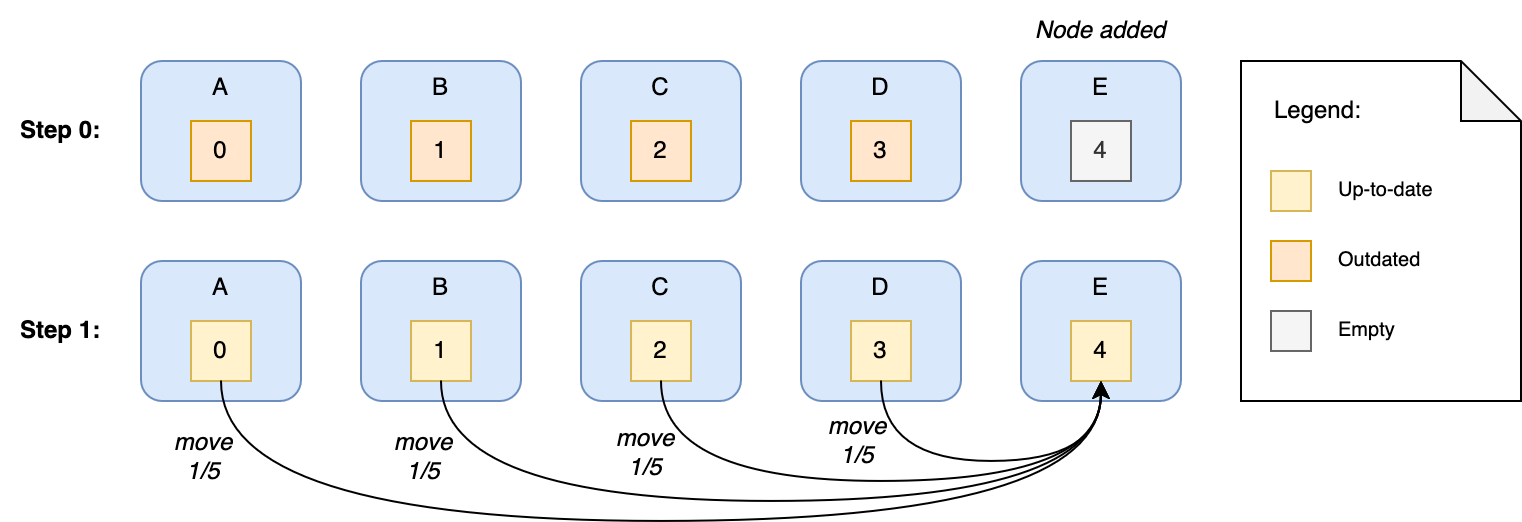
\includegraphics[width=0.8\linewidth]{img/diagram.png}
\caption{\label{fig:diagram}The Diagram Captions Are Also Title Case \cite{greenwade93}}
\end{figure}

A figure should appear in the same section it's referenced in, 
so be careful that Latex doesn't place it in the next section because it couldn't fit in the current one.
It can be placed before it is referenced though (I think, correct this if I'm wrong).
This is one reason why sections should span at least one page,
so that you have enough room to place the floating figures within it.
If your sections are too small, simply merge them.

Notice how figure \ref{fig:diagram} couldn't fit on the page right after the section title where it was defined,
so it was moved to the next page instead.
But now it's at the top of the page, which UTM doesn't allow.
So you have to move the definition of the figure somewhere else,
in this case after this paragraph.
Setting \verb|[!hb]| on the figure would make it go to the bottom of the page,
leaving a big gap between this text and the figure,
so that's not a solution.


\section{How to write Mathematics}

\LaTeX{} is great at typesetting mathematics. Let $X_1, X_2, \ldots, X_n$ be a sequence of independent and identically distributed random variables with $\text{E}[X_i] = \mu$ and $\text{Var}[X_i] = \sigma^2 < \infty$, and let Equation \ref{eq:sum}:
\begin{equation}
\label{eq:sum}
S_n = \frac{X_1 + X_2 + \cdots + X_n}{n}
      = \frac{1}{n}\sum_{i}^{n} X_i
\end{equation}
denote their mean. Then as $n$ approaches infinity, the random variables $\sqrt{n}(S_n - \mu)$ converge in distribution to a normal $\mathcal{N}(0, \sigma^2)$.


\section{How to add Citations and a References List}

You can simply upload a \verb|.bib| file containing your BibTeX entries, created with a tool such as JabRef. You can then cite entries from it, like this: \cite{greenwade93}. Just remember to specify a bibliography style, as well as the filename of the \verb|.bib|. You can find a \href{https://www.overleaf.com/help/97-how-to-include-a-bibliography-using-bibtex}{video tutorial here} to learn more about BibTeX.

If you have an \href{https://www.overleaf.com/user/subscription/plans}{upgraded account}, you can also import your Mendeley or Zotero library directly as a \verb|.bib| file, via the upload menu in the file-tree.


\section{Existing Solutions}

Here is an example of how to format a Table \ref{tbl:table1},
you might need it to compare existing solutions.
Formatting tables is probably the most difficult thing in Latex.


\begin{table}[H]
\caption{Example Table That Fits Page Width}
\label{tbl:table1}
\begin{tabularx}{\textwidth}{|Y|Y|Y|}
  \hline
  \textbf{Column 1} & \textbf{Column 2} & \textbf{Column 3} \\
  \hline
  Long wrapped content that fits nicely in the cell and breaks into multiple lines &
  Another wrapped text entry to demonstrate alignment &
  Final column with enough text to require wrapping too \\
  \hline
  Short entry & Medium text content here & More wrapped content \\
  \hline
\end{tabularx}
\end{table}
